\chapter{Related Work}

Nowadays, many scholars worldwide have submitted research projects relating to turning sign language into text, using a variety of methodologies and perspectives.

Which two main approaches can be mentioned as follows:
\begin{itemize}
  \item \textbf{Glove-based approaches:} This approach requires deaf and mute people to wear a sensor glove. When users have any different action or gesture, they record all those movements. After that, data from the sensor will analyze by the analyzer component and return the output to the user.
  \item \textbf{Vision-based approaches:} With this approach, developers will apply image processing algorithms to determine hand position, gestures, and hand movements. The user will not have to wear necessary glove-based methods, which is convenient. However, using image processing algorithms, we need to deal with the worst quality output, which these algorithms affect.
\end{itemize}

With a vision-based approach, early work used several image processing algorithms to build feature vectors based on a single RGB image of the hand. In this paper, "Real-time sign language recognition using a consumer depth camera" \cite{kuznetsova2013real}, using multi-layered random forest (MLRF) not only allows them to recognize hand signs correctly but also minimizes training time and effort. Alternatively, in this paper, "Sign Language Translation in Urdu/Hindi Through Microsoft Kinect," sign language can be recognized by auxiliary equipment: Microsoft Kinect (see figure \ref{fig:Chap2-MS-Kinect}), which captures the signs of the deaf person, after that, through the computer system, they can detect what do deaf people say.

\begin{figure}[H]
  \centering
  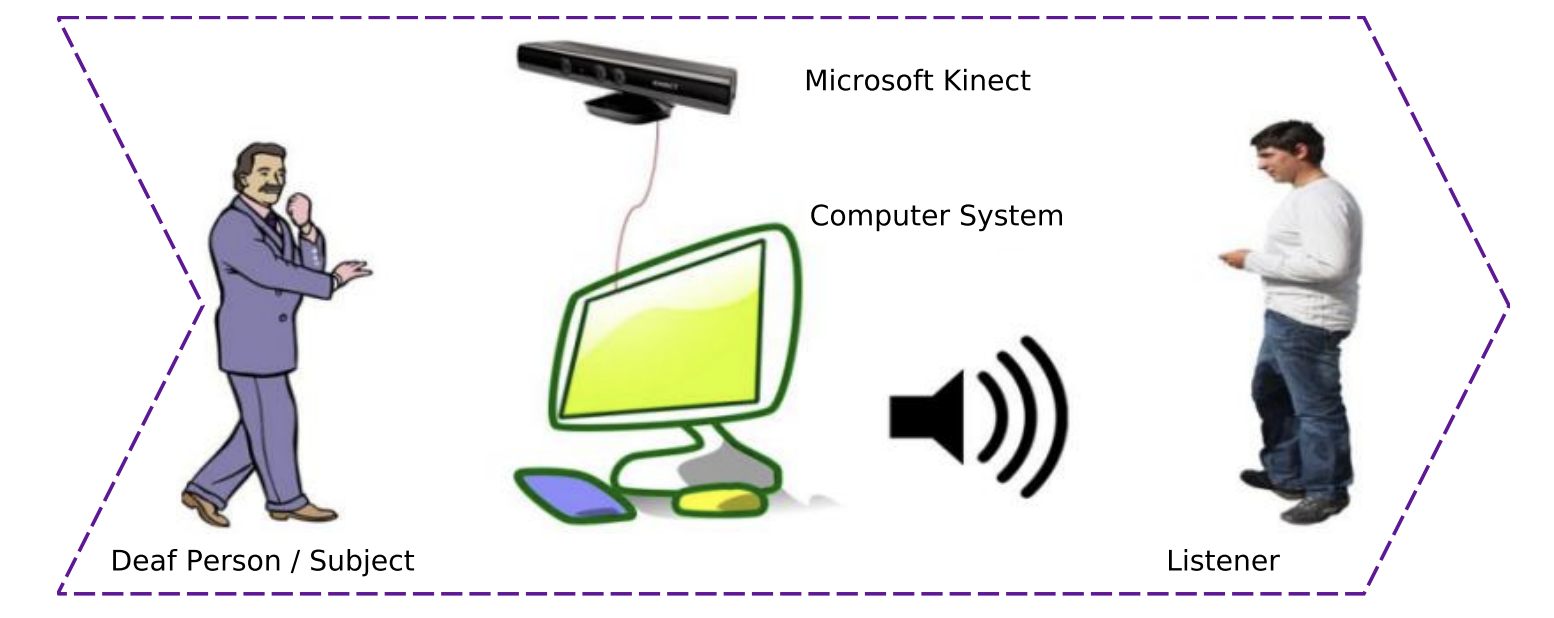
\includegraphics[width=\textwidth]{img/Chap2/MS-Kinect.png}
  \caption{Using Microsoft Kinect to translating sign language}
  \label{fig:Chap2-MS-Kinect}
\end{figure}

Besides the vision-based approach, glove based system has much relevant research. This paper, "The Language of Glove: Wireless gesture decoder with low-power and stretchable hybrid electronics" \cite{o2017language} introduces the way to convert American Sign Language (ASL) alphabet into text and display it on a computer or smartphone (see figure \ref{fig:Chap2-Glove-Base}). They can detect which hand gesture is performed with sensor gloves and send the result to a smartphone via Bluetooth. The sign language interprets text and displays it on the digital display screen. This approach is helpful in the real world for the deaf and mute who cannot converse with ordinary people.

\begin{figure}[H]
  \centering
  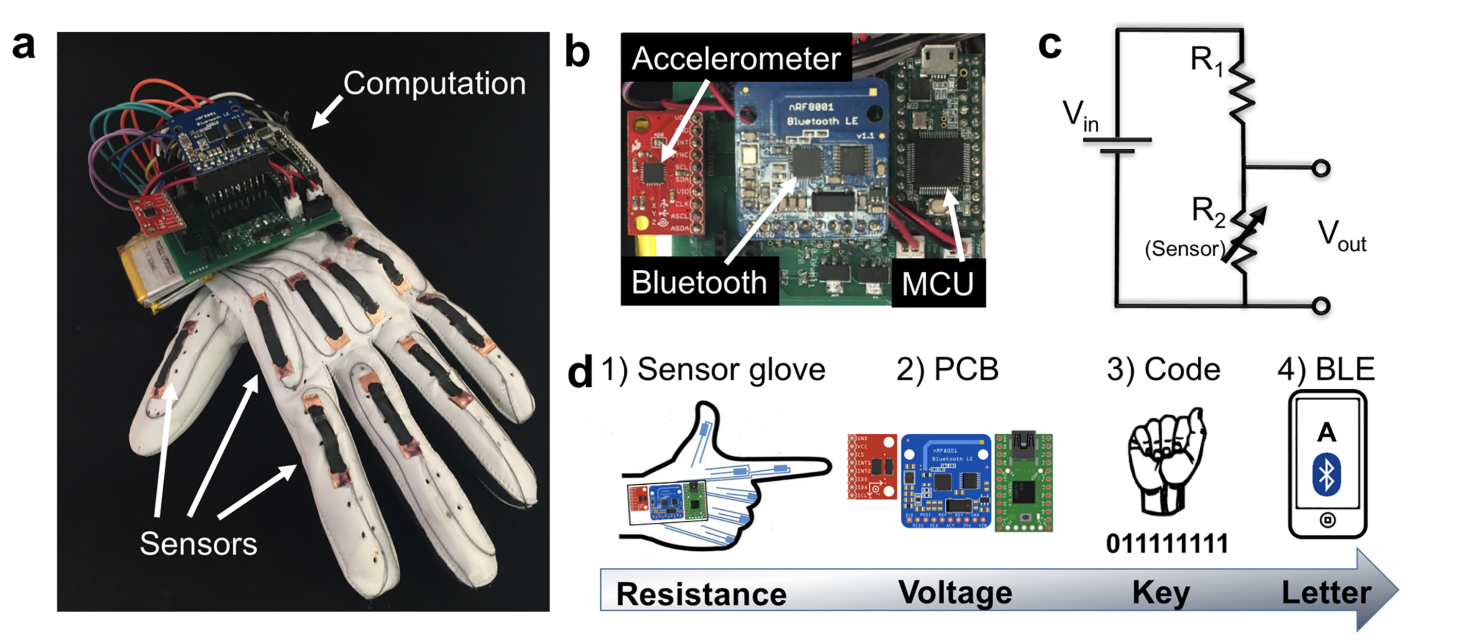
\includegraphics[width=\textwidth]{img/Chap2/Glove-Based.png}
  \caption{Glove based approach to translating sign language}
  \label{fig:Chap2-Glove-Base}
\end{figure}

Both approaches above have some problems; they can only recognize a minimal number of words, like an alphabet, number, or some word with easy hand shape and no motion. However, it is not easy; many words will use the same hand shape but differ in many characteristics, such as position and direction. There is currently no model that can handle the conversion of sign language flexibly and conveniently for the deaf and mute, helping them communicate effectively and naturally. Therefore, by applying appropriate technologies, the authors carry out this graduation thesis to break down the barriers between deaf and mute people and ordinary people, helping them become self-sufficient and more confident in daily communication.

